% \iffalse meta-comment
%<*internal>
\def\nameofplainTeX{plain}
\ifx\fmtname\nameofplainTeX\else
  \expandafter\begingroup
\fi
%</internal>
%<*install>
\input docstrip.tex
\keepsilent
\askforoverwritefalse
\preamble
Copyright (C) 2015,2016 by Barbara Bredner <bredner@bb-sbl.de>, 
Barbara Jentges <barbara.jentges@phact.ch> and 
Martin Sievers <martin.sievers@schoenerpublizieren.de>

This work may be distributed and/or modified under the
conditions of the LaTeX Project Public License (LPPL), either
version 1.3c of this license or (at your option) any later
version.  The latest version of this license is in the file:

http://www.latex-project.org/lppl.txt

This work is "maintained" (as per LPPL maintenance status) by
Barbara Bredner, Barbara Jentges and Martin Sievers.

This work consists of all files listed in manifest.txt.
\endpreamble
\postamble

\endpostamble

\usedir{tex/latex/pharmrep}
\nopostamble
\generate{
  \file{\jobname.cls}{\from{\jobname.dtx}{class}}
}
\nopreamble\nopostamble
\Msg{*********************************************************}
\Msg{*}
\Msg{* To finish the installation you have to move the}
\Msg{* following file into a directory searched by TeX:}
\Msg{*}
\Msg{* \space\space pharmrep.cls}
\Msg{*}
\Msg{* To produce the documentation run the file pharmrep.dtx}
\Msg{* through LaTeX (twice).}
\Msg{*}
\Msg{* \space\space makeindex -s gglo.ist -o pharmrep.gls pharmrep.glo}
\Msg{* \space\space makeindex -s gind.ist pharmrep.idx}
\Msg{*}
\Msg{* through makeIndex to produce the glossary. Finally, run PdfLaTeX once again.}
\Msg{*}
\Msg{* Das ist schon alles!}
\Msg{*}
\Msg{* Happy TeXing!}
\Msg{*********************************************************}
%</install>
%<install>\endbatchfile
%<*internal>
\usedir{source/latex/pharmrep}
\generate{
  \file{\jobname.ins}{\from{\jobname.dtx}{install}}
}
\nopreamble\nopostamble
\usedir{doc/latex/pharmrep}
\generate{
  \file{pharmrep-manual.tex}{\from{\jobname.dtx}{manual}}
  \file{pharmrep-manual.bib}{\from{\jobname.dtx}{manualbib}}
  \file{\jobname-template.tex}{\from{\jobname.dtx}{template}}
}
\ifx\fmtname\nameofplainTeX
  \expandafter\endbatchfile
\else
  \expandafter\endgroup
\fi
%</internal>
% \fi
%
% \iffalse
%<*driver>
\ProvidesFile{pharmrep.dtx}
%</driver>
%<class>\NeedsTeXFormat{LaTeX2e}[1999/12/01]
%<class>\ProvidesClass{pharmrep}
%<*class>
    [2016/04/12 v2.0 PharmRep -- a LaTeX package for medical reports]
%</class>
%<*driver>
\documentclass{ltxdoc}
\usepackage[a4paper,margin=25mm,left=50mm,nohead]{geometry}
\usepackage[numbered]{hypdoc}
\usepackage{blindtext}
\usepackage{siunitx}
\usepackage{booktabs}
\usepackage{ltablex}
%\usepackage{graphicx}
%\usepackage{tikz}
%\usepackage{caption}
\usepackage[babel]{csquotes}
%\usepackage{biblatex}
%\addbibresource{\jobname-template.bib}
%\usepackage{chemfig}
\usepackage{hyperref}
\hypersetup{%
   colorlinks = true,%
   allcolors  = blue,%
   breaklinks = true,%
   linktoc    = all,%
}
^^A\usepackage[nopostdot,nonumberlist,toc]{glossaries} 
^^A\setlength{\glspagelistwidth}{\linewidth}
^^A\usepackage{glossary-list}
^^A\setglossarystyle{list}
^^A\makenoidxglossaries
^^A\newglossaryentry{abb:eCTD}{name={eCTD},description={electronic Common Technical Document}}
^^A\newglossaryentry{abb:CTD}{name={CTD},description={Common Technical Document}}
^^A\newglossaryentry{abb:ICH}{name={ICH},description={International Conference on Harmonisation of Technical Requirements for Registration of Pharmaceuticals for Human Use}}
^^A\newglossaryentry{abb:URL}{name={URL},description={Universal Resource Locator}}
%
\EnableCrossrefs
\CodelineIndex
\RecordChanges
\providecommand*{\pkg}[1]{\textsf{#1}}
\begin{document}
  \DocInput{\jobname.dtx}
\end{document}
%</driver>
% \fi
%
% \CheckSum{0}
%
% \CharacterTable
%  {Upper-case    \A\B\C\D\E\F\G\H\I\J\K\L\M\N\O\P\Q\R\S\T\U\V\W\X\Y\Z
%   Lower-case    \a\b\c\d\e\f\g\h\i\j\k\l\m\n\o\p\q\r\s\t\u\v\w\x\y\z
%   Digits        \0\1\2\3\4\5\6\7\8\9
%   Exclamation   \!     Double quote  \"     Hash (number) \#
%   Dollar        \$     Percent       \%     Ampersand     \&
%   Acute accent  \'     Left paren    \(     Right paren   \)
%   Asterisk      \*     Plus          \+     Comma         \,
%   Minus         \-     Point         \.     Solidus       \/
%   Colon         \:     Semicolon     \;     Less than     \<
%   Equals        \=     Greater than  \>     Question mark \?
%   Commercial at \@     Left bracket  \[     Backslash     \\
%   Right bracket \]     Circumflex    \^     Underscore    \_
%   Grave accent  \`     Left brace    \{     Vertical bar  \|
%   Right brace   \}     Tilde         \~}
%
% \changes{v2.0}{2016/04/12}{First public release on Github}
%
% \GetFileInfo{\jobname.dtx}
% \DoNotIndex{\newcommand,\newenvironment}
%
% \title{\pkg{pharmrep} -- A \LaTeX{} package for Medical Reports\thanks{This file
%   describes version \fileversion, last revised \filedate.}
% }
% \author{Barbara Bredner\thanks{Email: bredner@bb-sbl.de}\and Barbara Jentges\thanks{Email: barbara.jentges@phact.ch}\and Martin Sievers\thanks{Email: martin.sievers@schoenerpublizieren.de}}
% \date{Released \filedate}
% \maketitle
%
% \begin{abstract}
% \noindent The class \pkg{pharmrep} provides a set of tools for authors of submission-relevant 
% documents in a consistent way. The package has an extended set of configuration options to make it 
% possible to .....
%
% \pkg{pharmrep} helps users to write standardised scientific pdf documents which have to be 
% sent (electronically) to authorities. The class setups a layout (page layout, fonts etc.) and  different 
% properties of the resulting output file (bookmarks, hyperlinks, tagging, fast web view etc.) to match given 
% requirements. In addition a template can be used as a starting point for new documents. 
% \end{abstract}
%
% \section{Installation}
% TODO:text for installation needs to be included here
% 
% <include general description about the package here>.
% 
% \subsection{Specific Packages included into PharmRep}
% The PharmRep package includes a number of other packages that facilitate edit scientific texts and 
% guarantee a level of harmonization throughout the complete submission-relevant documentation.
%
% \subsubsection{\pkg{siunitx} -- A Comprehensive (SI) Units Package}
%
% package \verb|siunitx|
%
% ``Physical quantities have both numbers and units, and each physical quantity should be expressed as the 
% product of a number and a unit. Typesetting physical quantities requires care to ensure that the 
% combined 
% mathematical meaning of the number-unit combination is clear. In particular, the SI units system 
% (International System of Units) lays down a consistent set of units with rules on how these are to be
% used. However, different countries and publishers have differing conventions on the exact appearance 
% of numbers (and units). The `siunitx` package provides a set of tools for authors to typeset quantities in a 
% consistent way.The package has an extended set of configuration options which make it possible to 
% follow 
% varying typographic conventions with the same input syntax. The
% package includes automated processing of numbers and units, and the ability to control tabular 
% alignment of numbers."
%
% In addition, numbers are automatically formatted.
%
% Example:
% TODO:description of siunitx and examples
%
% \subsubsection{hyperxmp -- Creating PDF 1b Format}
% <Hier kurze Beschreibung zum Package einfügen>.
%
% \section{Dealing with Typical Problems by using PharmRep}
% One typical problem that may occur when using Latex respectively the PharmRep package may occur, 
% when the PDF that was successfully compiled remains opened when further editing the tex-file. With the 
% PDF opened, the compilation process cannot be performed and the following error message apprears:
% MedRepStyle<xx>.tex: Fehler; Zeile 30: I can't write on file 'MedRepManual23.pdf' ..
% Once the PDF is closed, compilation can be performed without any problems.
%
% \section{User Feedback and Reporting Bugs}
% Feedback on PharmRep is always welcome and will help us in improving the package and correct any
% problems.
% <is there an 'official' chanel for reporting problems?
%
% \section{Thanks}
% We would like to express our particular thanks to Martin Sievers, who supported the development of
% the PharmRep with valuable input and tested the beta version, including identifying any incorrect output,
% bad documentation and spelling mistakes in the documentation. His specific focus was the support in
% solutions on how to create PDF/A-1b compatible files with the PharmRep package.
%
% \section{zu behebende Probleme}
% \begin{itemize}
%     \item Einbindung von externen Grafiken bzw. Tabellen macht Probleme, siehe TestPage.pdf (in der %Praxis: Einbindung von Plots, HPLC-Chromatogrammen, etc.)
%     \item Excel2Latex bei umfangreichen Tabellen mit Text über mehrere Zeilen ergibt Probleme
% \end{itemize}
%\StopEventually{^^A
%  \PrintChanges
%  \PrintIndex
%}
%
% \section{Implementation}
%
%    \begin{macrocode}
%<*class>
\RequirePackage{kvoptions}
\SetupKeyvalOptions {
   family  = pharmrep,%
   prefix  = pharmrep@,%
   setkeys = \kvsetkeys,%
}

\DeclareStringOption[utf8]{inputenc}
\DeclareStringOption[sRGB_IEC61966-2-1_black_scaled.icc]{colorprofile}
\DeclareBoolOption[true]{pdfa}
\DeclareBoolOption[false]{letter}
\DeclareVoidOption{US}{\pharmrep@lettertrue}
\ProcessKeyvalOptions*\relax
\PassOptionsToPackage{\pharmrep@inputenc}{inputenc}
%    \end{macrocode}
%    \begin{macrocode}
\RequirePackage{etoolbox}
%    \end{macrocode}
% For pdf 1.4 output and xml metadata
%    \begin{macrocode}
\RequirePackage{pdf14}
\input glyphtounicode.tex
\input glyphtounicode-cmr.tex
\pdfgentounicode=1
\pdfobjcompresslevel=0
\pdfinclusioncopyfonts=1 
%    \end{macrocode}
% Load KOMA documentclass scrartcl with required options
%    \begin{macrocode}
\ifpharmrep@letter
   \PassOptionsToPackage{paper=letter,pagesize}{typearea}
\fi%
\LoadClass[parskip=half,fontsize=12bp,%
      bibliography=totoc,listof=totoc,%
      numbers=noendperiod]{scrartcl}
%    \end{macrocode}
% pdf 1b format
%    \begin{macrocode}
\RequirePackage{hyperxmp}
%    \end{macrocode}
% Input encoding
%    \begin{macrocode}
\RequirePackage{inputenc}
%    \end{macrocode}
% Font encoding
%    \begin{macrocode}
\RequirePackage[T1]{fontenc}
   \hyphenchar\font=\string"7F
%    \end{macrocode}
% Language definition, typesetting and hyphenation
%    \begin{macrocode}
\RequirePackage[english]{babel} 
   \addto{\captionsenglish}{\renewcommand*{\contentsname}{Table of Contents}}
   \addto{\extrasenglish}{\def\figureautorefname{figure}}
   \addto{\extrasenglish}{\def\tableautorefname{table}}
   
%    \end{macrocode}
% Font evtl. TeXGyre einbinden, z.B. über eine Option
%    \begin{macrocode}
\RequirePackage{mathptmx} % times font
\RequirePackage{couriers} % monospace fonts
\RequirePackage[scaled=0.91]{helvet}   % for sans serif fonts (\textsf{...} or \sffamiliy)
\RequirePackage{pifont}   % symbols
\RequirePackage{textcomp} % symbols
\RequirePackage{microtype}% microtypographic extensions
\RequirePackage{xspace}   % automatic spacing with own commands
%    \end{macrocode}
% Graphic extensions
%    \begin{macrocode}
\RequirePackage{graphicx}
\RequirePackage{grffile}
%    \end{macrocode}
% Color profile
%    \begin{macrocode}
\RequirePackage[rgb]{xcolor}
\ifpharmrep@pdfa
   \IfFileExists{\pharmrep@colorprofile}
      {\immediate\pdfobj stream attr{/N 3}  file{\pharmrep@colorprofile}
      \pdfcatalog{%
      /OutputIntents [ <<
      /Type /OutputIntent
      /S/GTS_PDFA1
      /DestOutputProfile \the\pdflastobj\space 0 R
      /OutputConditionIdentifier (\pharmrep@colorprofile)
      /Info(\pharmrep@colorprofile)
      >> ]
      }}{\ClassError{pharmrep}{Color profile \pharmrep@colorprofile not found!}{Please check your installation}}
\else
   \ClassInfo{pharmrep}{PDF/A support is disabled!}
\fi%
%    \end{macrocode}
% SI number formatting
%    \begin{macrocode}
\RequirePackage{siunitx}
%    \end{macrocode}
% Page layout, header and footer
%    \begin{macrocode}
\RequirePackage{geometry}
    \geometry{textheight=600pt,head=50pt,left=60pt,right=60pt,includeheadfoot}
    \setlength{\footheight}{38pt}
\RequirePackage[section]{placeins}
\RequirePackage{lastpage}
\RequirePackage{totcount}
   \regtotcounter{figure}
   \regtotcounter{table}
\IfFileExists{scrlayer-scrpage.sty}
   {\RequirePackage[headsepline,footsepline]{scrlayer-scrpage}}%
   {\RequirePackage[headsepline,footsepline]{scrpage2}}%
   \setkomafont{pageheadfoot}{\small}
   \setkomafont{pagenumber}{\small}
   \clearscrheadfoot
    \ihead{\begin{minipage}[b][16mm]{0.48\textwidth}Applicant: \@Applicant\\Drug Product: 
    \@DrugProduct\hspace{0pt}\end{minipage}}
    \ohead{\begin{minipage}[b][16mm]{0.48\textwidth}\raggedleft\@PharmRepTitle\hspace{0pt}\end{minipage}}
    \ifoot{\begin{minipage}[t][10mm]{0.3\textwidth}\vspace{0pt}\@eCTDno\end{minipage}}
    \cfoot{\begin{minipage}[t][10mm]{0.3\textwidth}\vspace{0pt}\centering\jobname{}\end{minipage}}
    \ofoot{\begin{minipage}[t][10mm]{0.3\textwidth}\vspace{0pt}\flushright\pagemark/\upshape\pageref*{LastPage}\end{minipage}}
    \pagestyle{scrheadings}
%    \end{macrocode}
% Portrait- and Landscape-Format
%    \begin{macrocode}
\newcommand{\landscapeformat}{%
   \clearpage%
   \pdfpagewidth=\paperheight%
   \pdfpageheight=\paperwidth%
   \newgeometry{textwidth=600pt,left=50pt,top=60pt,bottom=60pt,includeheadfoot}}
\newcommand{\portraitformat}{%
   \clearpage%
   \pdfpagewidth=\paperwidth%
   \pdfpageheight=\paperheight%
   \restoregeometry}
%    \end{macrocode}
% Tables and figures
%    \begin{macrocode}
\renewcommand{\fps@table}{htbp}
\renewcommand{\fps@figure}{htbp}
\RequirePackage[justification=RaggedRight,singlelinecheck=false,labelfont=bf,hypcap=false]{caption}
\RequirePackage{rotating}
\RequirePackage{booktabs}
\RequirePackage{multirow}
\RequirePackage{ltablex}
%    \end{macrocode}
% Lists
%    \begin{macrocode}
\RequirePackage{enumitem}
   \setlist[1]{parsep=4pt}
%    \end{macrocode}
% Notes and comments
%    \begin{macrocode}
\RequirePackage[backgroundcolor=orange!40,%
    linecolor=black!20!orange,%
    textsize=footnotesize,%
    colorinlistoftodos]{todonotes}
   \reversemarginpar
   \setlength{\marginparwidth}{20mm}

\RequirePackage[babel]{csquotes}
%    \end{macrocode}
% Bibliography
%    \begin{macrocode}
\RequirePackage[backend=biber,%
   style=authoryear,%
   ]{biblatex}
\RequirePackage{xpatch}% author bold
   \xpretobibmacro{author}{\mkbibbold\bgroup}{}{}
   \xapptobibmacro{author}{\egroup}{}{}
   \xpretobibmacro{bbx:editor}{\mkbibbold\bgroup}{}{}
   \xapptobibmacro{bbx:editor}{\egroup}{}{}
   \renewcommand*{\labelnamepunct}{\mkbibbold{\addcolon\space}}
\AtEndPreamble{%
   \ifdefempty{\@BibFileName}{%
      \ClassError{pharmrep}{You have to provide a bib file!}{Please use the macro 
      \string\BibFileName{<MYFILE.bib>} in the preamble}}%
      {\addbibresource{\@BibFileName}}%
}%
%    \end{macrocode}
% Internal and external links, pdf meta data
%    \begin{macrocode}
\RequirePackage[pdftex,pdfa]{hyperref}%
   \AtEndPreamble{%
   \hypersetup{%
      pdftitle       = {\@PharmRepTitle},%
      pdfauthor      = {\@Applicant},%
      pdfsubject     = {\@eCTDno},%
      pdfkeywords    = {},%
      pdflang        = en,%
      bookmarks      = true,%
      pdfdisplaydoctitle = true,%
      plainpages     = false,%
      hypertexnames  = false,%
      pdfpagelabels  = true,%
      hyperindex     = true,%
      unicode        = true,%
      pdfmetalang    = {en},%
      pdfpagemode    = UseOutlines,% 
      bookmarksopen  = true,%
      bookmarksnumbered  = true, %
      bookmarksopenlevel = 2,%
      colorlinks         = true,%
      allcolors          = blue,%
      breaklinks         = true,%
      linktoc            = all,%
   }}%
\apptocmd{\UrlBreaks}{\do\f\do\m}{}{}
   \setcounter{biburllcpenalty}{9000}%
   \setcounter{biburlucpenalty}{9000}%
%    \end{macrocode}
% Glossary
%    \begin{macrocode}
\RequirePackage[nopostdot,nonumberlist,toc]{glossaries} 
   \setlength{\glspagelistwidth}{\linewidth}
\RequirePackage{glossary-list}
   \setglossarystyle{list}
   \makenoidxglossaries
%      \renewcommand{\glsnamefont}[1]{\bfseries #1}
%    \end{macrocode}
%    \begin{macrocode}
\setcounter{tocdepth}{4}
\setcounter{secnumdepth}{4}
%    \end{macrocode}
%    \begin{macrocode}
%%%\AtBeginDocument{\addto\extrasenglish{\def\figureautorefname{Abb.}}
%%%\addto\extrasenglish{\def\tableautorefname{table}}}
%%%\renewcaptionname{english}{\figureautorefname}{figure}
%%%\renewcaptionname{english}{\tableautorefname}{tab}
%    \end{macrocode}
%    \begin{macrocode}
\newcommand*{\@Applicant}{}
\newcommand*{\@DrugProduct}{}
\newcommand*{\@PharmRepTitle}{}
\newcommand*{\@eCTDno}{} 
\newcommand*{\@BibFileName}{}
\newcommand*{\Applicant}[1]{\renewcommand*{\@Applicant}{#1}}
\newcommand*{\DrugProduct}[1]{\renewcommand*{\@DrugProduct}{#1}}
\newcommand*{\PharmRepTitle}[1]{\renewcommand*{\@PharmRepTitle}{#1}}
\newcommand*{\eCTDno}[1]{\renewcommand*{\@eCTDno}{#1}}
\newcommand*{\BibFileName}[1]{\renewcommand*{\@BibFileName}{#1}}
%    \end{macrocode}
%    \begin{macrocode}
\AtBeginDocument{%
   \listoftodos % List of ToDo's if at least 1 \todo{xxx} is present in the document
   \clearpage
   
   \pdfbookmark[1]{\@PharmRepTitle}{Sec:Title}
   \section*{\@PharmRepTitle}
   \bigskip
   
   \tableofcontents
   \clearpage
   \ifnum\totvalue{table}>0
      \listoftables
      \clearpage
   \fi%
   \ifnum\totvalue{figure}>0
      \listoffigures
      \clearpage
   \fi%
   \cleardoubleemptypage
}%
%    \end{macrocode}
%    \begin{macrocode}
%</class>
%    \end{macrocode}
%\Finale
%
% \iffalse
%
%<*manual>
\documentclass{pharmrep}
\Applicant{Testpharma Inc.}
\DrugProduct{Master Mega Break Solution}
\PharmRepTitle{MedRep -- A Package to create eCTD-compliant PDFs}
\eCTDno{eCTD Sequence Number xxxx} 
\BibFileName{pharmrep-manual.bib} % Name of the bibliography file with extension .bib, e.g. biblio.bib

%% Examples Structural Formula
\usepackage{chemfig}

\usepackage{blindtext} % just for demonstration purposes
\usepackage{hologo}
\newcommand{\BibTeX}{\hologo{BibTeX}\xspace}
\newcommand{\biber}{\hologo{biber}\xspace}
\newcommand{\PharmRep}{\textsf{PharmRep}\xspace}
\makeatletter
\DeclareRobustCommand\meta[1]{%
   \ensuremath\langle
   \ifmmode \expandafter \nfss@text \fi
   {%
      \meta@font@select
      \edef\meta@hyphen@restore
      {\hyphenchar\the\font\the\hyphenchar\font}%
      \hyphenchar\font\m@ne
      \language\l@nohyphenation
      #1\/%
      \meta@hyphen@restore
   }\ensuremath\rangle
}
\DeclareRobustCommand\cs[1]{\texttt{\char`\\#1}}
\providecommand\marg[1]{%
   {\ttfamily\char`\{}\meta{#1}{\ttfamily\char`\}}}
\providecommand\oarg[1]{%
   {\ttfamily[}\meta{#1}{\ttfamily]}}
\providecommand\parg[1]{%
   {\ttfamily(}\meta{#1}{\ttfamily)}}
\def\meta@font@select{\itshape}

\newcommand{\pkg}[1]{\textsf{#1}}

\newcommand{\eg}{e.\,g.\xspace}
\makeatother

%% define entries for glossary: \newglossaryentry{<label>}{{<name/abbreviation>}{<brief description>}}
\newglossaryentry{abb:eCTD}{name={eCTD},description={electronic Common Technical Document}}
\newglossaryentry{abb:CTD}{name={CTD},description={Common Technical Document}}
\newglossaryentry{abb:ICH}{name={ICH},description={International Conference on Harmonisation of Technical Requirements for Registration of Pharmaceuticals for Human Use}}
\newglossaryentry{abb:URL}{name={URL},description={Universal Resource Locator}}

\begin{document}
\section{Introduction and Scope}
<hier weitere Hintergrundinformationen einfügen, z.B. strukturierte Dokumente / bookmarks in PDFs; 
ICH M4R3; eCTD Spec; FDA-PDF-Spec>
The current manual is structured and formatted according to a typical submission file that is planned to 
be included into an electronic dossier (either NeeS or eCTD) in portable document format (PDF). When 
creating a file by using \LaTeX, the manual should be read in connection with the respective 
\LaTeX{} template. 

If any specific formatting or style settings are required in the document in question (e.g. the need to 
create a table) the correct \LaTeX{} settings can be copy-pasted from the manual directly into this document.
The manual will be amended and updated on a regular basis.

\subsection{Formal Requirements for Submission-relevant Documents}
Minimum general requirements for layout and formatting of submission-relevant documents that form 
part of the Common Technical Document (CTD) are
given in the internationally harmonized document ICH M4 (R3) <Referenz einfügen> and the Q-A 
document: 

\subsection{Basic Requirements for Layout and Format}
\begin{itemize}
\item Text and tables should be prepared using margins that allow the document to be printed on 
both A4 paper (E.U. and Japan) and 8.5 x 11” paper (U.S.)
\item The left-hand margin should be sufficiently large that information is not obscured by the 
method of binding
\item Font sizes for text and tables should be of a style and size that are large enough to be easily 
legible, even after photocopying. Times New Roman, 12-point font, is recommended for narrative text
\item Every page should be numbered be starting at page one, except for individual literature 
references, where the existing journal page numbering is considered sufficient.
\item Acronyms and abbreviations should be defined the first time they are used in each module.
\item References should be cited in accordance with the current edition of the Uniform 
Requirements 
for Manuscripts Submitted to Biomedical Journals, International Committee of Medical Journal Editors 
(ICMJE)"
\item each page of a document should include a unique header or footer that briefly identifies its 
subject matter, an abbreviation of the full section number and title can be used. The applicant is free to 
put his logo on top of the CTD. However, logos are not acceptable in CTD sections' titles.
\item In order to avoid 5th, 6th etc. level subheading numbering (e.g. 2.6.6.3.2.1) within a document, 
the applicant can use a shortened numbering string. In this case, the document number and the name 
(\eg 2.6.6 Toxicology Written Summary) should appear in page headers or footers and then section 
numbering within the document can be used, for example, 1, 1.1, 2, 3, 3.1, 3.2 etc. Use of the full numbering string 
(\eg 2.6.6.3.2.1) is also considered acceptable.
\end{itemize}

\subsection{Additional Settings that need to be considered for Portable Document Files}
With the eCTD becoming the mandatory format of a dossier in the major industrial regions of the world, 
specific settings in the PDF documents as addressed in the ICH eCTD specification <include reference 
here> 
need to be considered in the submission-relevant documents. Additional regional settings may need to 
be 
considered as addressed in the region-specific Module 1 eCTD specifications.

\section{Short Description about the Features of \PharmRep}
PharmRep is a 'ready-to-use' package for creating eCTD-compliant PDFs with high-level layout that is 
harmonized all over the submission files created with \PharmRep. \PharmRep uses the format settings as 
required for submission relevant documents with view to becoming eCTD-PDFs. Once compiled, only 
minor PDF-settings need to be completed in ADOBE (\eg `initial view', etc as addressed in chapter xx of the 
present document). 

The \PharmRep package was especially developed for \LaTeX{} beginners. It has been developed with view to 
optimizing the creation of submission-relevant documents in a time-efficient way with focus on content 
without loosing time 


\section{Instructions for the Users of \PharmRep Package}
<hier kurze allgemeine Erläuterung einfügen; inbesondere der Hinweis, dass das Package für 
LaTex-Anfänger gedacht ist, die ohne erfahrene LaTex-User zu sein, mit Hilfe des Packages hochwertig 
formatierte Zulassungsdokumente erzeugen wollen. In diesem Sinne mögen Hinweise aus dem Kapitel 
Instructrions for the Users of PharmRep - insbesondere auch die im Anhang bereitgestellte short list of 
comman commands überflüssig erscheinen.

\subsection{Section Levels and Section Numbering}
Numbering of sections, subsections and subsubsections is added automatically during the compilation.

%% \todo{4 numbered levels are required}
The numbering is indicated by the command \cs{section} for title level 1, \cs{subsection} for level 2, 
\cs{subsubsection} for level 3, and \cs{paragraph} for level 4. 
Please note: Only the `section', `subsection',\dots titles will be automatically converted to bookmarks during 
the PDF creation.

For paragraphs, text is usually in the same layout as the title, but a paragraph is not numbered. The 
unnumbered `paragraph' levels will not be converted to bookmarks during the PDF creation. 
\begin{itemize}
   \item Level 1 Title 1: sections: \verb|\section{Title}|
   \item Subtitle 1.1 level 2 - Sub-Title 1.1: subsections: \verb|\subsection{Title}|
   \item Section level 3 -- Subsub-Title 1.1.1: subsubsections: \verb|\subsubsection{Title}|
   \item Section level 4 -- ParagraphTitle : paragraph: \verb|\paragraph{Title}|
   \item Section level 5 -- Sub-ParagraphTitle : subparagraph: \verb|\subparagraph{Title}|
\end{itemize}

\subsection{Page Orientation: Portrait and Landscape}
\blindtext

\landscapeformat
\subsubsection{Landscape}
\verb|\landscapeformat|

\blindtext

\blindtext

\portraitformat
\subsubsection{Back to Portrait}
\verb|\portraitformat|

\blindtext

\subsection{Common Formatting Functions}
\subsubsection{Paragraphs and Line Breaks}
\begin{itemize}
   \item new paragraph: insert 1 or more blank line(s)  (more than 1 will be ignored during the 
   compilation
   \item new line or line break: \verb|\newline|
\end{itemize}

\subsubsection{Hyphenation}
\begin{itemize}
   \item separate words: \verb| | 1 or more blanks (more than 1 will be ignored during the compilation)
   \item no break between two words: \verb|~|
   \item enable hyphenation at specific locations of a word: \verb|\-| (\eg \verb|reac\-tion|) Usually not necessary since hyphenation is already enabled by the loaded packages
\end{itemize}

\subsubsection{Quotation Marks}
\begin{itemize}
   \item quotation mark (``double'') \verb|``double''| 
   \item quotation mark (`single') \verb|`single'| \todo{Hint to csquotes}
\end{itemize}

\subsubsection{Font Style}
\begin{itemize}
   \item \textbf{bold} text: \verb|\textbf{text}|
   \item \textit{italic} text: \verb|\textit{text}|
   \item {\small small text}: \verb|{\small small text}|
   \item {\footnotesize footnotesize text}: \verb|{\footnotesize footnotesize text}|
   \item {\tiny tiny text}: \verb|{\tiny tiny text}| (usually too small)
\end{itemize}

\subsubsection{Special Characters}
In most cases a backslash (\textbackslash) directly in front of a special character will work, \eg
\begin{itemize}
   \item \% (percent): \verb|\%|
   \item \& (ampersand): \verb|\&|
\end{itemize}

\subsection{Annotations in a tex-file}
Annotations in the TeX{} file may be used for explanatory purposes -- or as a reminder that specific 
information is still missing and needs to be included into the document.
Annotations only appear in the \TeX{} file, the are not converted into the PDF.

Symbol for annotations in the \TeX{} file is \verb| %| (everything in a line after a \% is ignored)

\subsection{Tables}
In \LaTeX{}, `table' is the name for a floating object (see p.~\pageref{subsubsec:TableFloating}), whereas 
`tabular' provides the environment for tables. In a `tabularx' environment, the table width can be set (\eg 
to \cs{textwidth}) and page breaks are enabled \footnote{for \PharmRep the package \pkg{ltablex} is used}.
Creating tables with \LaTeX{} require some experience. In the following, basic instructions on how to create 
tables are described. Alternatively, tables can be created in MS~Excel and converted into \LaTeX{} tables by 
installing the Excel-add-in Excel2Latex. Tables can also be included as objects.

\subsubsection{Caption of Tables}
Every table included into a document requires a brief, informative title ('caption') that describes its 
contents in nonsentence format <Let.Ref. ACS Style Guide>.  Tables are numbered sequentially with 
arabic numerals. 

Please make sure that every table needs to be discussed within the text, whereas the tables should be 
discussed sequentially, so that Table 1 is discussed before Table 2, Table 2 before Table 3, and so on 
<ACS Style Guide>.

A table caption should be placed at the beginning of the table.

Please note that the word ``Table'' is only capitalized when it is followed by the table number -- and in the 
beginning of the table caption that starts with ``Table'', followed by its numeral.

Each table with a caption is automatically listed in the list of tables.

\subsubsection{General layout options for tables}
\begin{verbatim}
The instructions as given below create a basic table with two columns and three row. In general, columns 
are separated by the symbol \& (ampersand) and rows are ended by using the command 
\textbackslash\textbackslash (double backslash). The column format is defined at the beginning of the 
table, e.g. \verb|{rr}| for two right-aligned columns (more options see \autopageref{tab:TabGenLayout}).

\captionof{table}{first tabular}\label{tab:FirstTab}
\begin{tabular}{rr}
a & 1 \\ 
b & 2 \\ 
c & 3 \\
\end{tabular}
\end{verbatim}

As an example, the instructions as given above create \autoref{tab:FirstTab} with two columns and three 
rows.
\begin{minipage}{\linewidth}
   \captionof{table}{first tabular}\label{tab:FirstTab}
   \begin{tabular}{rr}
      a & 1 \\ 
      b & 2 \\ 
      c & 3 \\
   \end{tabular}
\end{minipage}

The layout of a table can be modified with a huge number of commands and tools. The major 
characteristics of a table are the number and type of columns and lines. \autoref{tab:TabGenLayout} 
shows some of the options using the following code:
\begin{verbatim}
\begin{minipage}{\linewidth}%
\captionof{table}[xyz]{Some Options for tables}\label{tab:TabGenLayout}
\begin{tabularx}{\linewidth}{rlcp{10mm}S}\toprule
\textbf{Col 1} & \textbf{ Col 2} & \textbf{Col 3} &
\textbf{Col 4} & \textbf{ Col 5} \\ \cmidrule{1-4}
right & left & centered & fixed width &
\text{justified at decimal separator} \\ \midrule
& & & & 12.97 \\ 
& & & & 0.4 \\ 
& & & & 10000.3 \\ \bottomrule
\end{tabularx}
\end{minipage}%
\end{verbatim}

that results in the following PDF-printout: 

\begin{minipage}{\linewidth}
   \captionof{table}[xyz]{Some Options for tables}\label{tab:TabGenLayout}
   \begin{tabular}{rlcp{10mm}S}\toprule
      \textbf{Col 1} \texttt{r} & \textbf{ Col 2} \texttt{l} & \textbf{Col 3} \texttt{c} & \textbf{Col 4} 
      \texttt{p} & \textbf{ Col 5} \texttt{S} \\ \cmidrule(lr){1-4}
      right & left & centered & fixed width & \text{justified at decimal separator} \\ \midrule
      & & & & 12.97 \\ 
      & & & & 0.4 \\ 
      & & & & 10000.3 \\ \bottomrule
   \end{tabular}%
\end{minipage}

\bigskip

\subsubsection{General Commands for Table Layout}
In the follwing, general commands for typical table layout is given.

\paragraph{Column without and with Linebreak}

\begin{description}
   \item[Column] \textbf{formats}
   \begin{description}
      \item[without] \textbf{linebreak}
      \begin{description}
         \item[\texttt{r}] aligned right
         \item[\texttt{l}] aligned left
         \item[\texttt{c}] centered
         \item[\texttt{S}] justified at decimal separator
      \end{description}
      \item[with] \textbf{linebreak}
      \begin{description}
         \item[\texttt{p{<width>}}] parbox (`paragraph box') with predefined width
         \item[\texttt{X}] only in \texttt{tabularx} environment: parbox with flexible width to meet 
         the 
         predefined tablewidth (e.g. \verb|{\linewidth}|) 
      \end{description}
   \end{description}
   
   \paragraph{Long Table: Same Header and Footer on every Page}	
   \item[Header] \textbf{and footer} (example see p.~\pageref{subsubsec:longtables}\,ff.)
   \begin{description}
      \item[\cs{endhead\oarg{optional argument}}] table content before this command 
      will 
      be used for the header on every page of a table
      \item[\cs{endfoot\oarg{optional argument}}] table content between 
      \cs{endhead} and \cs{endfoot} will be used for the footer on 
      every page of a table. The footer is defined at the beginning of a table!
   \end{description}
   
   \paragraph{Table Lines - Horizontal and Vertical}	
   \item[Lines] Use horizontal lines rarely and avoid vertical lines always. Reasons and examples see \eg 
   \href{http://ctan.org/pkg/booktabs}{http://ctan.org/pkg/booktabs}
   \begin{description}
      \item[horizontal] \textbf{lines} (avoid whenever possible)
      \begin{description}
         \item[\cs{toprule}] first horizontal line at the top of the table
         \item[\cs{midrule}] horizontal line within the table
         \item[\cs{midrule\{a-b\}}] horizontal line starting at column \texttt{a} 
         and ending at column \texttt{b}
         \item[\cs{midrule(lr)\{a-b\}}] horizontal line starting at column \texttt{a} 
         and 
         ending at column \texttt{b} shortened left (\texttt{l}) and right (\texttt{r})
         \item[\cs{bottomrule}] last horizontal line at the end of the table
      \end{description}
      \item[vertical] \textbf{lines} Vertical lines in tables should be avoided in general. (They are easy 
      to use in \LaTeX, but a huge challenge regarding the readability and usability of any document.)
   \end{description}%
\end{description}%

\newpage

\subsubsection{Long Table -- Portrait Format}\label{subsubsec:longtables}
% Table generated by Excel2LaTeX from sheet 'Tabelle2'
\captionof{table}{Example long table}\label{tab:longtable} %\nopagebreak[1]
\begin{tabularx}{\linewidth}{lcrX}
   \toprule
   \textbf{Col 1} &  \textbf{Col 2} &  \textbf{Col 3} & \textbf{Col 4 with very long header using some more 
      superfluous additional text} \\\midrule\endhead 
   \midrule
   \textit{Foot 1} & \textit{Foot 2} & \textit{Foot 3} & \textit{Foot 4} \\\bottomrule\endfoot
   the   & 1    & a     & more and more text \\ \midrule
   quick & 2     & b     & some more text \\ \midrule
   brown & 3     & c     & some more text (in addition) \\ \midrule
   fox   & 4     & d     & more text \\ \midrule
   jumps & 5     & e     & more text \\ \midrule
   over  & 6     & f     & more text \\ \midrule
   the   & 7     & g     & more text \\ \midrule
   lazy  & 8     & h     & more text \\ \midrule
   dog   & 9     & i     & more text \\ \midrule
   .     & 10    & j     & more text \\ \midrule
   the   & 11    & k     & more and more text \\ \midrule
   quick & 12    & l     & some more text \\ \midrule
   brown & 13    & m     & some more text (in addition) \\ \midrule
   fox   & 14    & n     & more text \\ \midrule
   jumps & 15    & o     & more text \\ \midrule
   over  & 16    & p     & more text \\ \midrule
   the   & 17    & q     & more text \\ \midrule
   lazy  & 18    & r     & more text \\ \midrule
   dog   & 19    & s     & more text \\ \midrule
   .     & 20    & t     & more text \\ \midrule
   the   & 21    & u     & more and more text \\ \midrule
   quick & 22    & v     & some more text \\ \midrule
   brown & 23    & w     & some more text (in addition) \\ \midrule
   fox   & 24    & x     & more text \\ \midrule
   jumps & 25    & y     & more text \\ \midrule
   over  & 26    & z     & more text \\ \midrule
   the   & 27    & a     & more text \\ \midrule
   lazy  & 28    & b     & more text \\ \midrule
   dog   & 29    & c     & more text \\ \midrule
   .     & 30    & d     & more text \\ \midrule
\end{tabularx}

\newpage

\landscapeformat
\subsubsection{Long Table - Landscape Format}
% Table generated by Excel2LaTeX from sheet 'Tabelle2'
\captionof{table}{Example long table on a landscape page}\label{tab:longtableLandscape}
\begin{tabularx}{\textwidth}{lcrX}
   \toprule
   \textbf{Col 1} &  \textbf{Col 2} &  \textbf{Col 3} & \textbf{Col 4 with very long header using some more 
      superfluous additional text and extra words to stretch the tabular width to textwidth} \\ 
   \midrule\endhead 
   \midrule
   Foot 1 & Foot 2 & Foot 3 & Foot 4 \\\bottomrule\endfoot
   the   & 21    & u     & more and more text \\ \midrule
   quick & 2     & b     & some more text \\ \midrule
   brown & 3     & c     & some more text (in addition) \\ \midrule
   fox   & 4     & d     & more text \\ \midrule
   jumps & 5     & e     & more text \\ \midrule
   over  & 6     & f     & more text \\ \midrule
   the   & 7     & g     & more text \\ \midrule
   lazy  & 8     & h     & more text \\ \midrule
   dog   & 9     & i     & more text \\ \midrule
   .     & 10    & j     & more text \\ \midrule
   the   & 11    & k     & more and more text \\ \midrule
   quick & 12    & l     & some more text \\ \midrule
   brown & 13    & m     & some more text (in addition) \\ \midrule
   fox   & 14    & n     & more text \\ \midrule
   jumps & 15    & o     & more text \\ \midrule
   over  & 16    & p     & more text \\ \midrule
   the   & 17    & q     & more text \\ \midrule
   lazy  & 18    & r     & more text \\ \midrule
   dog   & 19    & s     & more text \\ \midrule
   .     & 20    & t     & more text \\ \midrule
   the   & 21    & u     & more and more text \\ \midrule
   quick & 22    & v     & some more text \\ \midrule
   brown & 23    & w     & some more text (in addition) \\ \midrule
   fox   & 24    & x     & more text \\ \midrule
   jumps & 25    & y     & more text \\ \midrule
   over  & 26    & z     & more text \\ \midrule
   the   & 27    & a     & more text \\ \midrule
   lazy  & 28    & b     & more text \\ \midrule
   dog   & 29    & c     & more text \\ \midrule
   .     & 30    & d     & more text \\ \midrule
\end{tabularx}

\portraitformat

\subsubsection{Table Footnotes}
<include instructions here>

\subsubsection{Positioning of Tables -- Floating versus Manually}\label{subsubsec:TableFloating}
In \LaTeX, tables and figures can basically be positioned in two different ways: They are included manually 
and appear exactly at this place (like in word processing software, \eg Microsoft Word) or they can be 
included as a floating object.

\paragraph{Floating Table}
Floating objects are included where they are in the code if there is enough space for a eye-friendly 
layout. In case the place is too small floating objects are positioned automatically near the original 
insertion. `Near' can be on the same page, the next page or farer away depending on the amount of text 
and/or other floating objects. Floating provides a more professional layout and should be used if 
possible 
to increase the readability.
\begin{table}[hbpt]
   \begin{tabular}{ccc}\toprule
      A & B & C \\\midrule 
      1 & has & 6 \\ 
      2 & a yellow & 4 \\ 
      3 & car & 2 \\\bottomrule
   \end{tabular} 
   \caption[short caption table]{Table as a floating object}\label{tab:tableFloatingObject}
\end{table}

Code for table \ref{tab:tableFloatingObject} (page \pageref{tab:tableFloatingObject})
\begin{verbatim}
\begin{table}[hbpt]
\begin{tabular}{ccc}\toprule
A & B & C \\\midrule 
1 & has & 6 \\ 
2 & a yellow & 4 \\ 
3 & car & 2 \\\bottomrule
\end{tabular} 
\caption[short caption table]{Table as a floating object}%
\label{tab:tableFloatingObject}
\end{table}
\end{verbatim}

printed in list of tables as ``\ref{tab:tableFloatingObject} {\color{blue}short caption table}'' . The 
optional short title \verb|[short caption table]| in squared brackets is used for LOT.  If no short title is 
given the whole caption is printed in the list of tables.

referred to by using:\newline
\verb|table \ref{tab:tableFloatingObject}| (result: table \ref{tab:tableFloatingObject}) or \newline
\verb|\autoref{tab:tableFloatingObject}| (result: \autoref{tab:tableFloatingObject}) 

page number:\newline
\verb|page \pageref{tab:tableFloatingObject}| (result: page \pageref{tab:tableFloatingObject}) or 
\newline
\verb|\autopageref{tab:tableFloatingObject}| (result: \autopageref{tab:tableFloatingObject})


\subsubsection{In-Text References to Tables}
In general, the instruction \verb|\label{key}| is used for names and references of tables, figures and 
everything else (e.g. sections, paragraphs). 

If a table or figure is included directly at a specific place a caption is included by

\verb|\captionof{figure}[short]{title}\label{fig:figurelabel}| or \newline
\verb|\captionof{figure}[short]{title}\label{tab:tablabel}| 

For floating tables or figures in a floating environment \verb|\begin{table}...\end{table}| (see 
\ref{subsubsec:TableFloating}) or \verb|\begin{figure}...\end{figure}| (see \ref{subsubsec:FigureFloating}): 

\verb|\caption[short]{title}\label{fig:figurelabel}| or \newline
\verb|\caption[short]{title}\label{tab:tablabel}|

\verb|[short]|: optional `short caption' being printed in the list of figures or list of tables, respectively, 
and `title' used for the figure or table itself. The label is used for reference purposes, \eg

\verb|\ref{fig:figurelabel}| or \verb|\ref{tab:tablabel}|

Label names do not work with special characters (except `:') or blanks.

\subsubsection{MS Excel Add-in 'Excel2LaTeX'}
Excel spreadsheets can be converted into a \LaTeX{} tabular structure manually or using third party 
software, \eg Excel2LaTeX (available on \url{http://www.ctan.org/pkg/excel2latex}).

Excel2LaTeX works for Windows, Mac OS X and Excel~2000 up to Excel~2010. For Excel~2007 and 
Excel~2010 the add-in has to be activated within the options menu in Excel. After a restart of Excel and 
the 
activation of `Excel2LaTeX' as a secure macro the add-in excel2latex is available in the ribbon `Add-In'.
<diese Angaben müssen noch auf Korrektheit geprüft werden; ggfs. hier keine weiteren Angaben, 
sondern nur Referenz auf das package, wo in der readme alle weiteren Details beschrieben sind>.

Instead of converting Excel or Word tables (and other parts) into \LaTeX the part could be included using 
\verb|\includegraphics| (see p.\pageref{sec:includepdfs}). <hier: Hinweis auf Vorgehensweise, wenn 
PDF/A-1b gefordert ist>.

\newpage
\subsection{Figures}
Figures are not directly inserted into the \TeX{} file, but are created as separate files which are included 
during the compilation. For PDF generation, file formats png, jpg or pdf are allowed, all others will 
produce an error.The figure-files need to be stored in the same folder as the \TeX{} file (alternatively, the complete 
file-path has to be provided). 

\subsubsection{Caption of Figures}
Every figure included into a document requires a brief, informative title ('caption') that describes its 
contents in nonsentence format <Let.Ref. ACS Style Guide>.  Figures are numbered sequentially with 
arabic 
numerals. 
Please make sure that every figure needs to be discussed within the text, whereas the figures should be 
discussed sequentially, so that Figure 1 is discussed before Figure 2, Figure 2 before Figure 3, and so on 
<ACS Style Guide>.

A figure caption should be placed below the figure.

Please note that the word ``Figure'' is only capitalized when it is followed by the figure number - and in 
the beginning of the figure caption that starts with Figure, followed by its numeral.

Each figure with a caption is automatically listed in the list of figures.

\subsubsection{Positioning of Figures -- Floating versus Manual}\label{subsubsec:FigureFloating}
\paragraph{Automatic Insertion of Figures (`Floating Figures')}
\begin{figure}[hbpt]
   
\includegraphics[width=0.2\linewidth]{ctanlion}
   \caption[short caption figure]{Figure as a floating object. CTAN lion drawing by Duane Bibby; thanks to \url{www.ctan.org}}
   \label{fig:figureFloatingObject}
\end{figure}

Code for figure \ref{fig:figureFloatingObject} (page~\pageref{fig:figureFloatingObject})
\begin{verbatim}
\begin{figure}[hbpt]

\includegraphics[width=0.2\linewidth]{ctanlion}
\caption[short caption figure]{Figure as a floating object. CTAN lion drawing by Duane Bibby; thanks to \url{www.ctan.org}}
\label{fig:figureFloatingObject}
\end{figure}
\end{verbatim}


printed in list of tables as ``\ref{fig:figureFloatingObject} {\color{blue}short caption figure}'' . The 
optional short title in squared brackets \verb|[short caption figure]| is used for LOF.  If no short title is 
given the complete caption is printed in the list of figures.

referred to by using:\newline
\verb|figure \ref{fig:figureFloatingObject}| (result: figure \ref{fig:figureFloatingObject}) or \newline
\verb|\autoref{fig:figureFloatingObject}| (result: \autoref{fig:figureFloatingObject}) 

page number:\newline
\verb|page \pageref{fig:figureFloatingObject}| (result: page \pageref{fig:figureFloatingObject}) or 
\newline
\verb|\autopageref{fig:figureFloatingObject}| (result: \autopageref{fig:figureFloatingObject})


\paragraph{Manual Insertion of Figures}\label{subsubsec:FigureManualInserted}
\begin{minipage}[t]{\linewidth}%
   
\includegraphics[width=0.2\linewidth]{ctanlion}
   \captionof{figure}{example of a manually inserted figure}%
   \label{fig:figureManuallyInserted}
\end{minipage}%

Code for figure \ref{fig:figureManuallyInserted} (page \pageref{fig:figureManuallyInserted})
\begin{verbatim}
\begin{minipage}[t]{\linewidth}%

\includegraphics[width=0.2\linewidth]{ctanlion}
\captionof{figure}{example of a manually inserted figure}%
{\label{fig:figureManuallyInserted}}
\end{minipage}%
\end{verbatim}

Note: It is recommended to end the \verb|\begin{minipage}| and \verb|\end{minipage}| line with a 
percent sign (\%) to avoid spurious blanks.

\subsubsection{In-Text References to Figures}
\verb|\label{key}| is used for names and references of tables, figures and everything else (\eg sections, 
paragraphs). 

If a table or figure is included directly at a specific place a caption is included by

\verb|\captionof{figure}[short]{title}\label{fig:figurelabel}| or \newline
\verb|\captionof{figure}[short]{title}\label{tab:tablabel}| 

A table caption should be placed at the beginning of the table whereas a figure caption is usually 
beneath the figure.

For floating tables or figures in a floating environment \verb|\begin{table}...\end{table}| (see 
\ref{subsubsec:TableFloating}) or \verb|\begin{figure}...\end{figure}| (see \ref{subsubsec:FigureFloating}): 

\verb|\caption[short]{title}\label{fig:figurelabel}| or \newline
\verb|\caption[short]{title}\label{tab:tablabel}|

\verb|[short]|: optional `short caption' being printed in the list of figures or list of tables, respectively, 
and `title' used for the figure or table itself. The label is used for reference purposes, \eg

\verb|\ref{fig:figurelabel}| or \verb|\ref{tab:tablabel}|

Label names do not work with special characters (except `:') or blanks.

\subsection{Footnotes in Text}
Footnotes are set by including \verb|\footnote{text}| directly behind the word, where the footnote 
should be added. No space should be placed between word and instruction. The footnote will be 
automatically numbered and placed at the end of the page. 

\subsection{Lists and Enumeration Items}
Lists can be described with different enumeration items. Generally, bullet points, numbered and 
description are used.

Reference of lists (only useful for page number reference since lists do not have a number/internal 
counter):
Define unique label using\newline
\verb|\label{list:listdescription}| \newline
Label names do not work with special characters (except `:') or blanks.

\subsubsection{Bullet Point Lists}
\begin{itemize}
   \item item 1
   \item item 2
\end{itemize}

Code for bullet point list:
\begin{verbatim}
\begin{itemize}
   \item item 1
   \item item 2
\end{itemize}
\end{verbatim}

\subsubsection{Numbered List}
\begin{enumerate}
   \item item 1
   \item item 2
\end{enumerate}

Code for numbered list:
\begin{verbatim}
\begin{enumerate}
   \item item 1
   \item item 2
\end{enumerate}
\end{verbatim}

\subsubsection{Description List}
\begin{description}
   \item[description label 1] item 1
   \item[description label 2] item 2
\end{description}

Code for description list:
\begin{verbatim}
\begin{description}
   \item[description label 1] item 1
   \item[description label 2] item 2
\end{description}
\end{verbatim}

\subsubsection{List in a List}
Lists can be combined arbitrarily and levels are automatically formatted, \eg bullet point and numbered 
list:
\begin{itemize}
\item item 1
\begin{enumerate}
\item subitem 1
\item subitem 2
\begin{itemize}
\item subsubitem 1
\item subsubitem 2
\end{itemize}
\item subitem 3
\end{enumerate}
\item item 2
\end{itemize}

Code for the combined list:
\begin{verbatim}
\begin{itemize}
   \item item 1
   \begin{enumerate}
      \item subitem 1
      \item subitem 2
      \begin{itemize}
         \item subsubitem 1
         \item subsubitem 2
      \end{itemize}
      \item subitem 3
   \end{enumerate}
   \item item 2
\end{itemize}
\end{verbatim}

\subsection{Splitting Large Documents}
Large documents can be split into several \verb|*.tex| files. Special characters should be avoided in the 
PDF file name!. For an example see below:

\begin{itemize}
\item three files: \verb|master.tex|, \verb|part1.tex| and \verb|part2.tex|
\item \verb|master.tex|: usual \LaTeX{} file with definition of styles, commands, etc.
\item \verb|part1.tex|, \verb|part2.tex|: two files with content which is copy-pasted into 
\verb|master.tex| using \verb|\input|
\end{itemize}

Typical commands for splitting documents are the following: <Kommandozeilen sind nicht klar, sollten 
besser erläutert werden>.

\begin{minipage}{\linewidth}
\begin{verbatim}
%%% master.tex file:

% preamble, styles, etc.
[...]

\begin{document}
some text
\input{part1.tex}
more text
\input{part2.tex}
some more text
\end{document}
\end{verbatim}
\end{minipage}


\subsection{Including Figures from external PDFs into the \LaTeX{} File}\label{sec:includepdfs}
Pictures, figures, tables and any other objects that are provided in PDF-files can be included into \LaTeX{} 
by using the command \cs{includegraphics\oarg{options}\marg{filename}}. Special characters and spaces should be avoided 
in the PDF file name!
\par\bigskip

Example
\begin{itemize}
\item The figure of the PDF-file \verb|pdfexample.pdf| is planned to be included into the file 
\verb|master.tex| 
\item \verb|master.tex|: usual \LaTeX file with definition of styles, commands, etc.
\item \verb|pdfexample.pdf|: pdf file
\end{itemize}

\begin{minipage}{\linewidth}%
{\small
\begin{verbatim}
%% master.tex file:

preamble, styles, etc.
[...]

\begin{document}
some text
\begin{minipage}{\linewidth}%
\captionof{figure}{example including pdf}
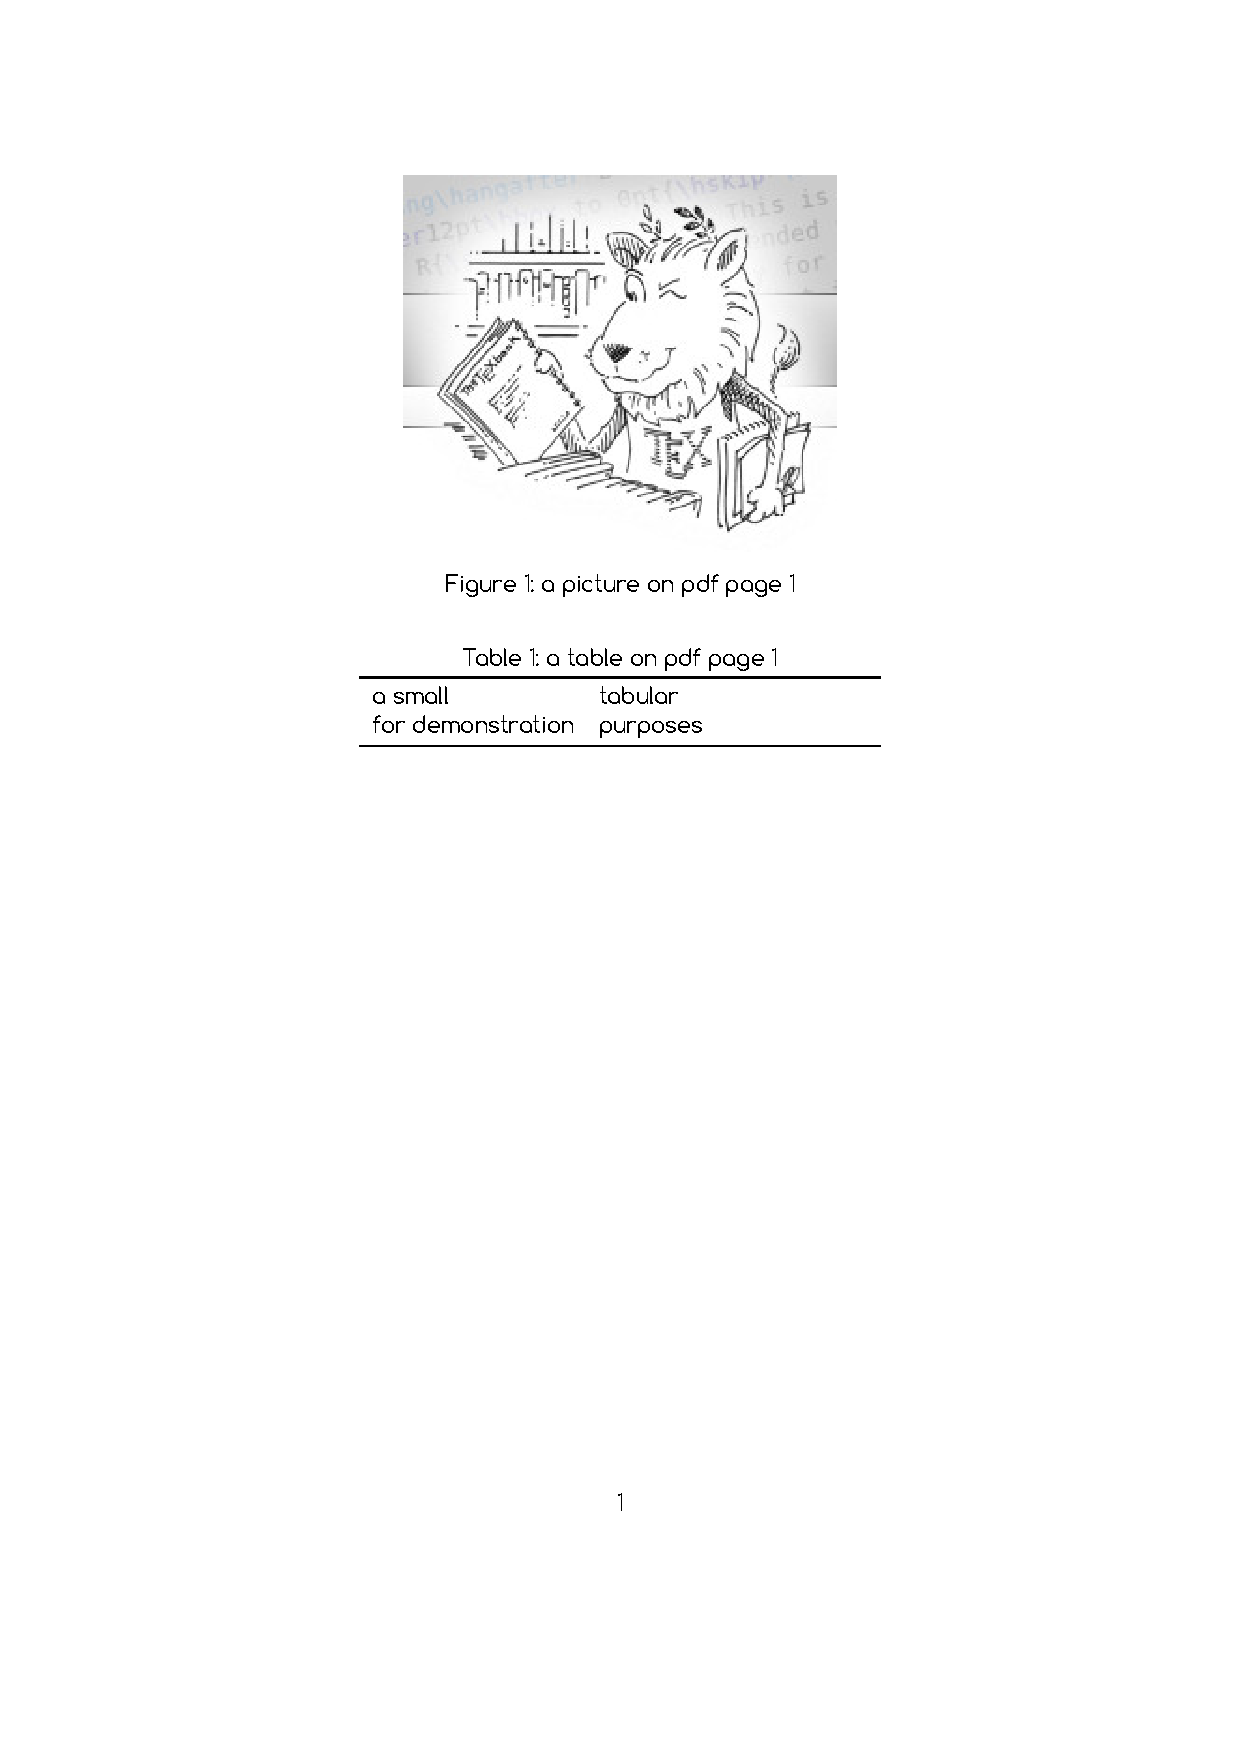
\includegraphics[page=1, trim=60mm 170mm 90mm 40mm, clip]{pdfexample.pdf}
\end{minipage}%
more text
\end{document}
\end{verbatim}%
}
\end{minipage}%
\bigskip

\subsubsection{Clipping of PDF Page}
Clipping of PDF pages is done via \verb|trim=<left> <top> <right> <bottom>| (with arbitrary units, \eg 
mm, pt) and (mandatory!) \verb|clip|.

<nicht klar, was hier passiert>.

<NOTE: if a PDF/A-1b document is required, the external PDF needs to be PDF/A-1b compliant itself. This 
can be created from other files (e.g. MS WORD, MS VISIO,etc) by using the 'print as' function and 
choosing 
in the PDF-properties the setting to create a PDF/A-1b-compatible PDF>.
\begin{figure}[htb]
\centering
\fcolorbox{blue}{white}{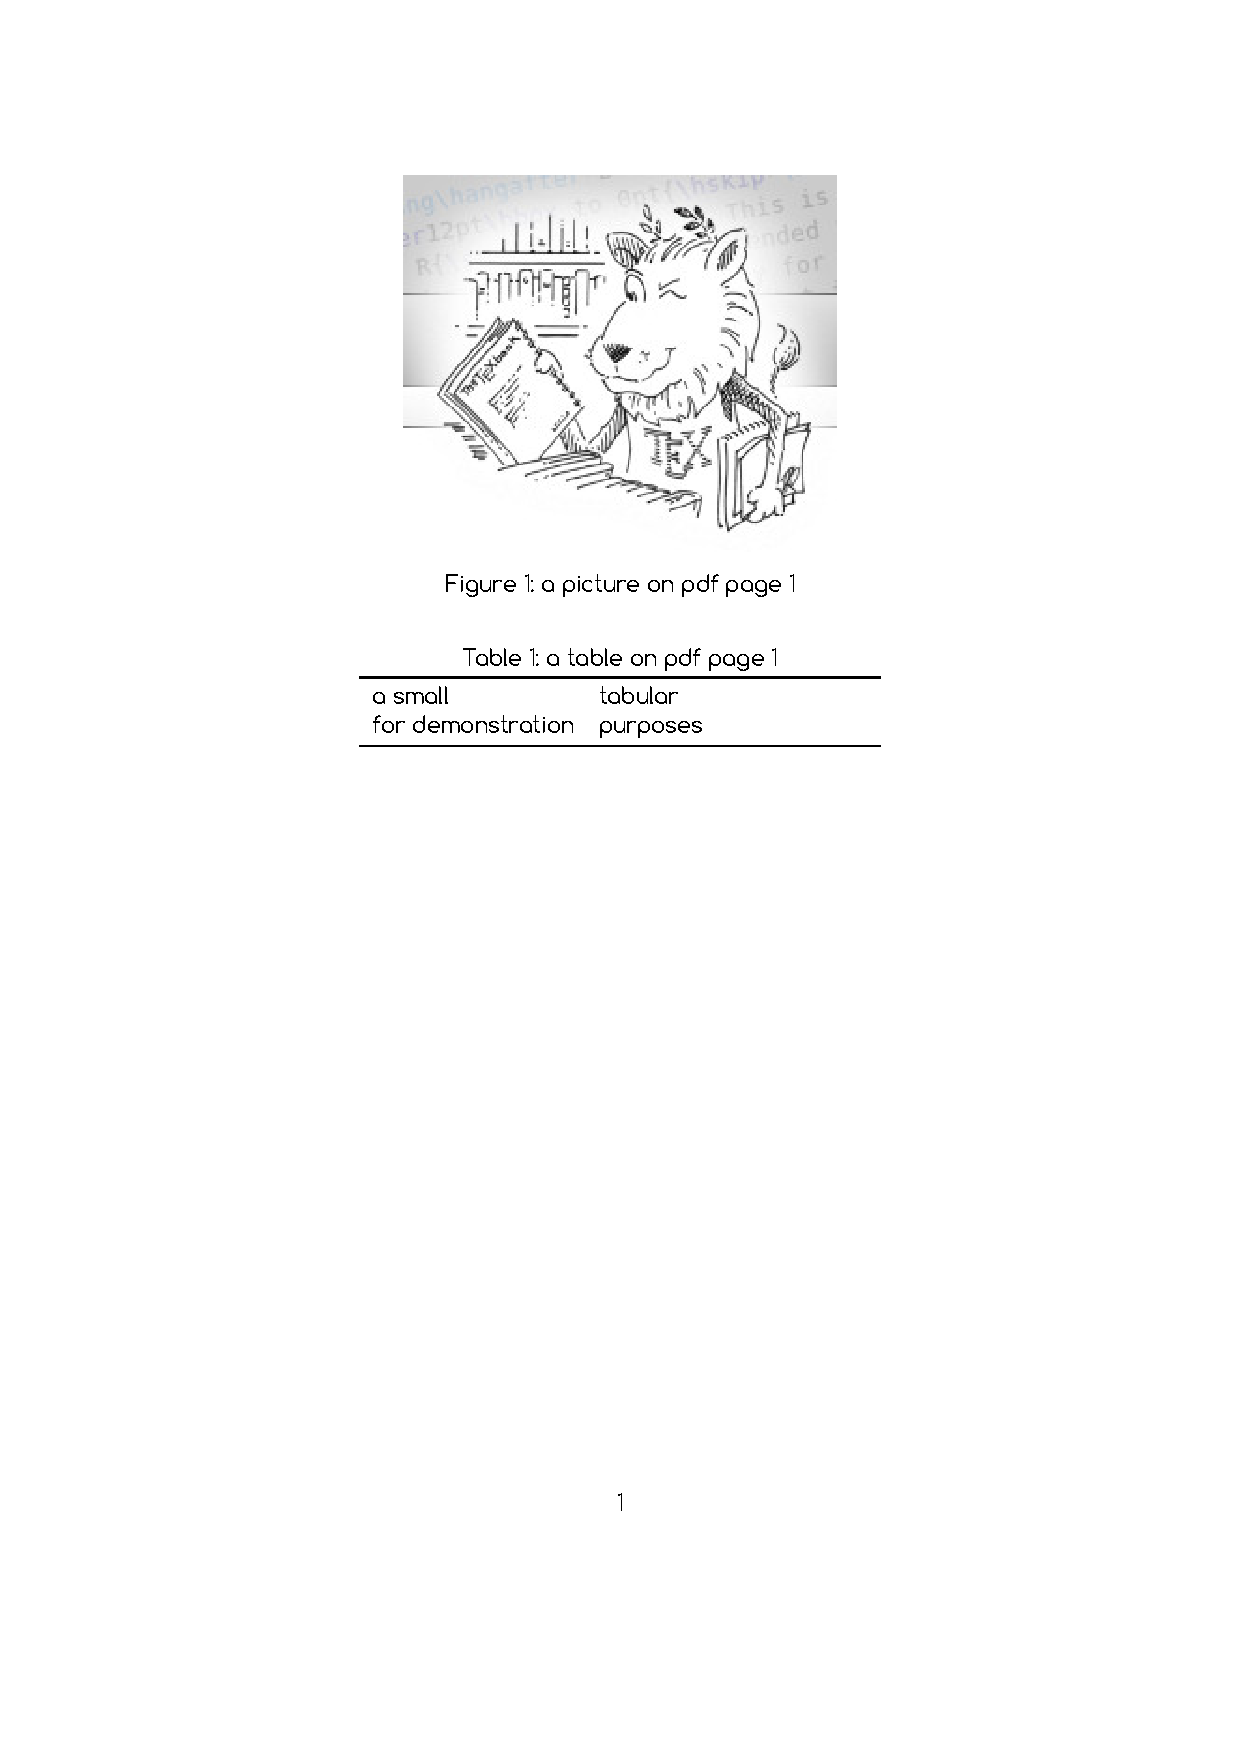
\includegraphics[page=1,trim = 60mm 170mm 90mm 40mm,clip]{pdfexample.pdf}}
\caption[example including pdf]{example including pdf (colored box for demonstration purposes)}
\end{figure}%

\subsection{Commenting in \TeX{} files}
A practical tool during the creation of a document is the inclusion of comments into the \TeX{} files. This 
may serve as reminders, remaining action items or comments required during document review.

\todo{a comment in the margin}Comments can be included with \verb|\todo{text}| for comments in the 
margin and \verb|[inline]{text}| for comments in the text. Do not use \verb|\todo|-comments within other %environments (e.g. figures, tables, etc.)
\todo[inline, color=green]{a green inline comment}
\begin{verbatim}
\todo{a comment in the margin}
\todo[inline, color=green]{a green inline comment}
\end{verbatim}
If at least one \verb|\todo|-command is present in the text the `list of todonotes' will be printed using
\verb|\listoftodos|.

\subsection{Bibliography with JabRef and Citations}
\subsubsection{Extenal Bibliography with JabRef}
External sources (books, papers, websites, etc.) are stored in a separate file \verb|literatur.bib|. bib-files
can be created using JabRef (\href{http://jabref.sourceforge.net/}{jabref.sourceforge.net/}), online and
versions for local installation available).
Example \verb|literatur.bib|:{\footnotesize
\begin{verbatim}
...
@ELECTRONIC{Q1E,%
author = {{International Conference on Harmonization}},%
shorthand = {{International Conference on Harmonization (2004)}},%
month = {6},%
year = {2004},%
title = {Guidance for Industry: Q1E Evaluation of Stability Data.},%
url = {http://www.fda.gov/RegulatoryInformation/Guidances/ucm128092.htm},%
urldate = {2014-06-28},%
owner = {Jane Doe},%
}%
@BOOK{Krishnamoorthy,%
title = {Statistical Tolerance Regions},%
shorthand = {Statistical Tolerance Regions (2009)}%
publisher = {Wiley},%
year = {2009},%
author = {Kalimuthu Krishnamoorthy and Thomas Mathew},%
isbn = {9780470380260},%
owner = {Jane Doe},%
timestamp = {2014-05-13},%
totalpages = {461}%
}
...
\end{verbatim}}

The bibliography entries are sorted during the compilation of the bibliography. This has to be done
separately and in addition to the text compilation (\eg in TeXstudio key \verb|F8| or \verb|F11|for bibliography and
key~\verb|F6| for text compilation). Tool for generating \BibTeX entries, \eg
\href{http://lead.to/amazon/en/}{http://lead.to/amazon/en/} (uses Amazon data base) and
\href{http://literatur-generator.de/}{http://literatur-generator.de/} (uses google). It doesn't matter if the
bib-file contains more bibliography entries than the tex-file; only cited sources are listed in the 
bibliography.

Test: \href{http://amazon.com}{Amazon.com}
% 
Note: The configuration for TeXstudio has to be changed that \biber is used for the bibliography (see figure~\ref{fig:TeXStudioBiber}).%
\begin{figure}[htb]
\centering
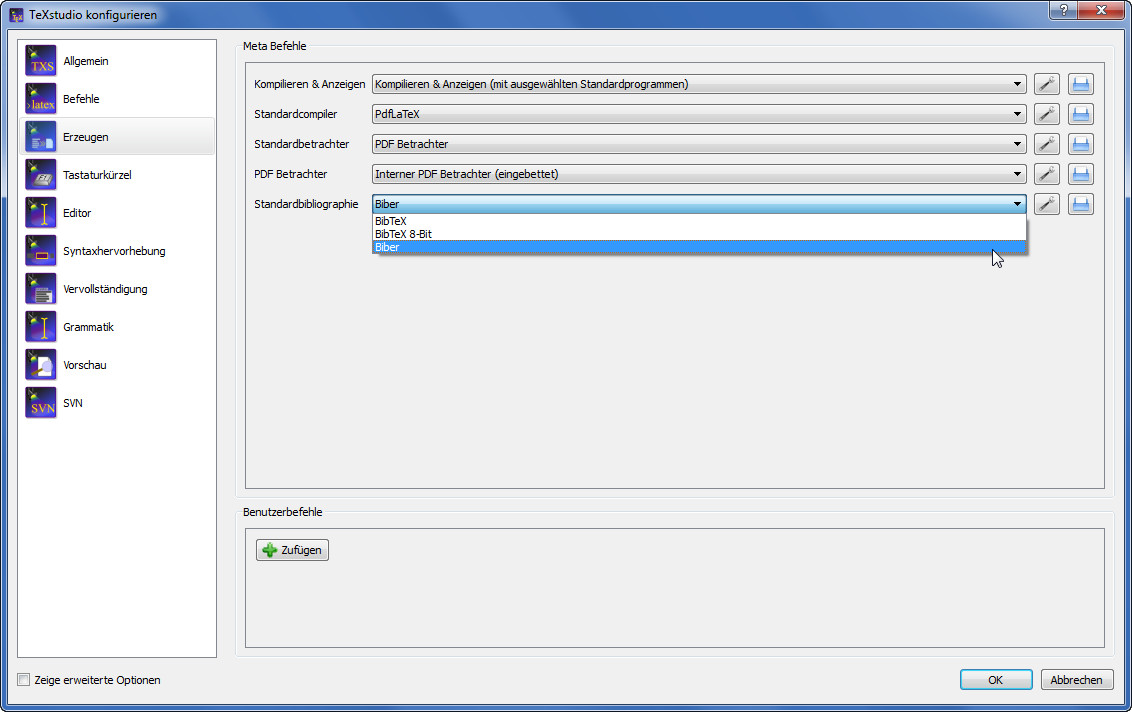
\includegraphics[width=\linewidth]{TeXStudioBiber}%
\caption{Configuration for \biber in TeXstudio}
\label{fig:TeXStudioBiber}
\end{figure}

\subsubsection{Citations}
All citations use the unique key for a bibliographical entry, \eg \verb|Q1E| or \verb|Krishnamoorthy|.%
using \verb|\cite{Q1E}|: \cite{Q1E}\\%
using \verb|\cite[123]{Q1E}|: \cite[123]{Q1E}\\%
using \verb|\cite[123--125]{Q1E}|: \cite[123--125]{Q1E}\\%
using \verb|\autocite{Q1E}|: \autocite{Q1E}\\%
using \verb|text\footcite{Q1E}|: text\footcite{Q1E}\\%
using \verb|\fullcite{Q1E}|: \fullcite{Q1E}\\%
Print all bibliographic entries cited in the text (independent of the entries in the bibliography file) with a numbered section:%
\verb|\printbibliography|%
\printbibliography%

\subsubsection{In-text Use of Universal Resource Locators (URLs)}
A Universal Resource Locator \gls{abb:URL} (which is the path to a certain file on the World Wide Web)
can be included directly into the text on two different ways:
\begin{itemize}
\item by including the instruction \verb|\url{URL}| Inhalt...
\item with different descriptive text or url: \verb|\href{URL}{text}|
\end{itemize}

Examples:%
\verb|\url{http://ctan.org}| \url{http://ctan.org}

\verb|\href{http://ctan.org}{ctan.org}| \href{http://ctan.org}{ctan.org}

\subsection{Creating a `List Abbreviations, Acronyms and Symbols'}\label{sec:glossary}
Abbreviations, acronyms and symbols that are used within the text need to be pre-defined  in the
preamble <where exactly?>, \eg\\
\verb|\newglossaryentry{abb:eCTD}|\newline
\hspace*{2em}\verb|{name={eCTD},|\newline
\hspace*{2em}\verb|description={electronic Common Technical Document}}|

After an abbreviation has been defined in the preamble, it can be used in the following text, e.g.
using \verb|\gls{abb:eCTD}|: \gls{abb:eCTD}

using \verb|\gls{abb:CTD}|: \gls{abb:CTD}

using \verb|\gls{abb:ICH}|: \gls{abb:ICH}

Used abbreviations, their explanation and page number(s) where they are used within the text are
automatically listed if a glossary is printed:\\
\verb|\printnoidxglossary[title={List of Abbreviations}]|

\todo{differentiation between separate 'List of Abbreviations' and 'Glossary' foreseen?}

\subsection{Setting intra-text Cross-References}
Define unique label using\newline
\verb|\label{sec:secdescription}|\newline
Label names do not work with special characters (except `:') or blanks.

Labels can be used everywhere (sections, paragraphs, figures, tables,...)

\section{Handling Specific Issues}
\subsection{How to create PDF/A-1b Files}
\todo{description to convert arbitrary graphs and documents (e.g. powerpoint slides) into pdf/a documents using printer functionality}
\todo{other useful things for pdf/a compatibility using Acrobat Professional}

\section{Organization of Different Types of Files used by \LaTeX{} in an eCTD File and Folder Structure}
\todo{an BB: Diesen Abschnitt bitte auf Korrektheit prüfen}
\LaTeX{} uses a number of file types. For details, reference is made to relevant \LaTeX{} publications, \eg
Frank Mittelbach, Michel Goossens, Der LaTeX Begleiter.
Some basic information about the different types of files, however, is required, in order to correctly
organize these files when creating documents that are
planned to be organized in an eCTD file and folder structure.

<hier: Auszug aus Tab. 1.1 von Mittelbach/Goossens einfügen>.

With reference to different ``texwelt'' discussions in this field,the question on how to handle the auxiliary
files that are created when creating \TeX{} and the corresponding PDF files, shall be addressed in this subsection.
In summary, and in order to enable a correct and smooth PDF creation, it can be concluded that the auxiliary files are recommended to be listed together with the \TeX{} files in one and the same folder and or sub-folder.

For further information, please find the respective discussions listed below:\\ \url{http://texwelt.de/wissen/fragen/2530/was-sind-hilfsdateien-und-wo-finde-ich-diese}

\url{http://texwelt.de/wissen/fragen/5501/wie-kann-ich-mit-latex-dateien-hilfsdateien-ordnern-ordnung-halten}
\url{http://tex.stackexchange.com/a/11125}
\url{http://tex.stackexchange.com/a/24787}

In this respect, it is recommended to created sub-folders for each CTD-related submission-file as given in \autoref{fig:eCTDstructure}.
\begin{figure}[hbpt]
\centering
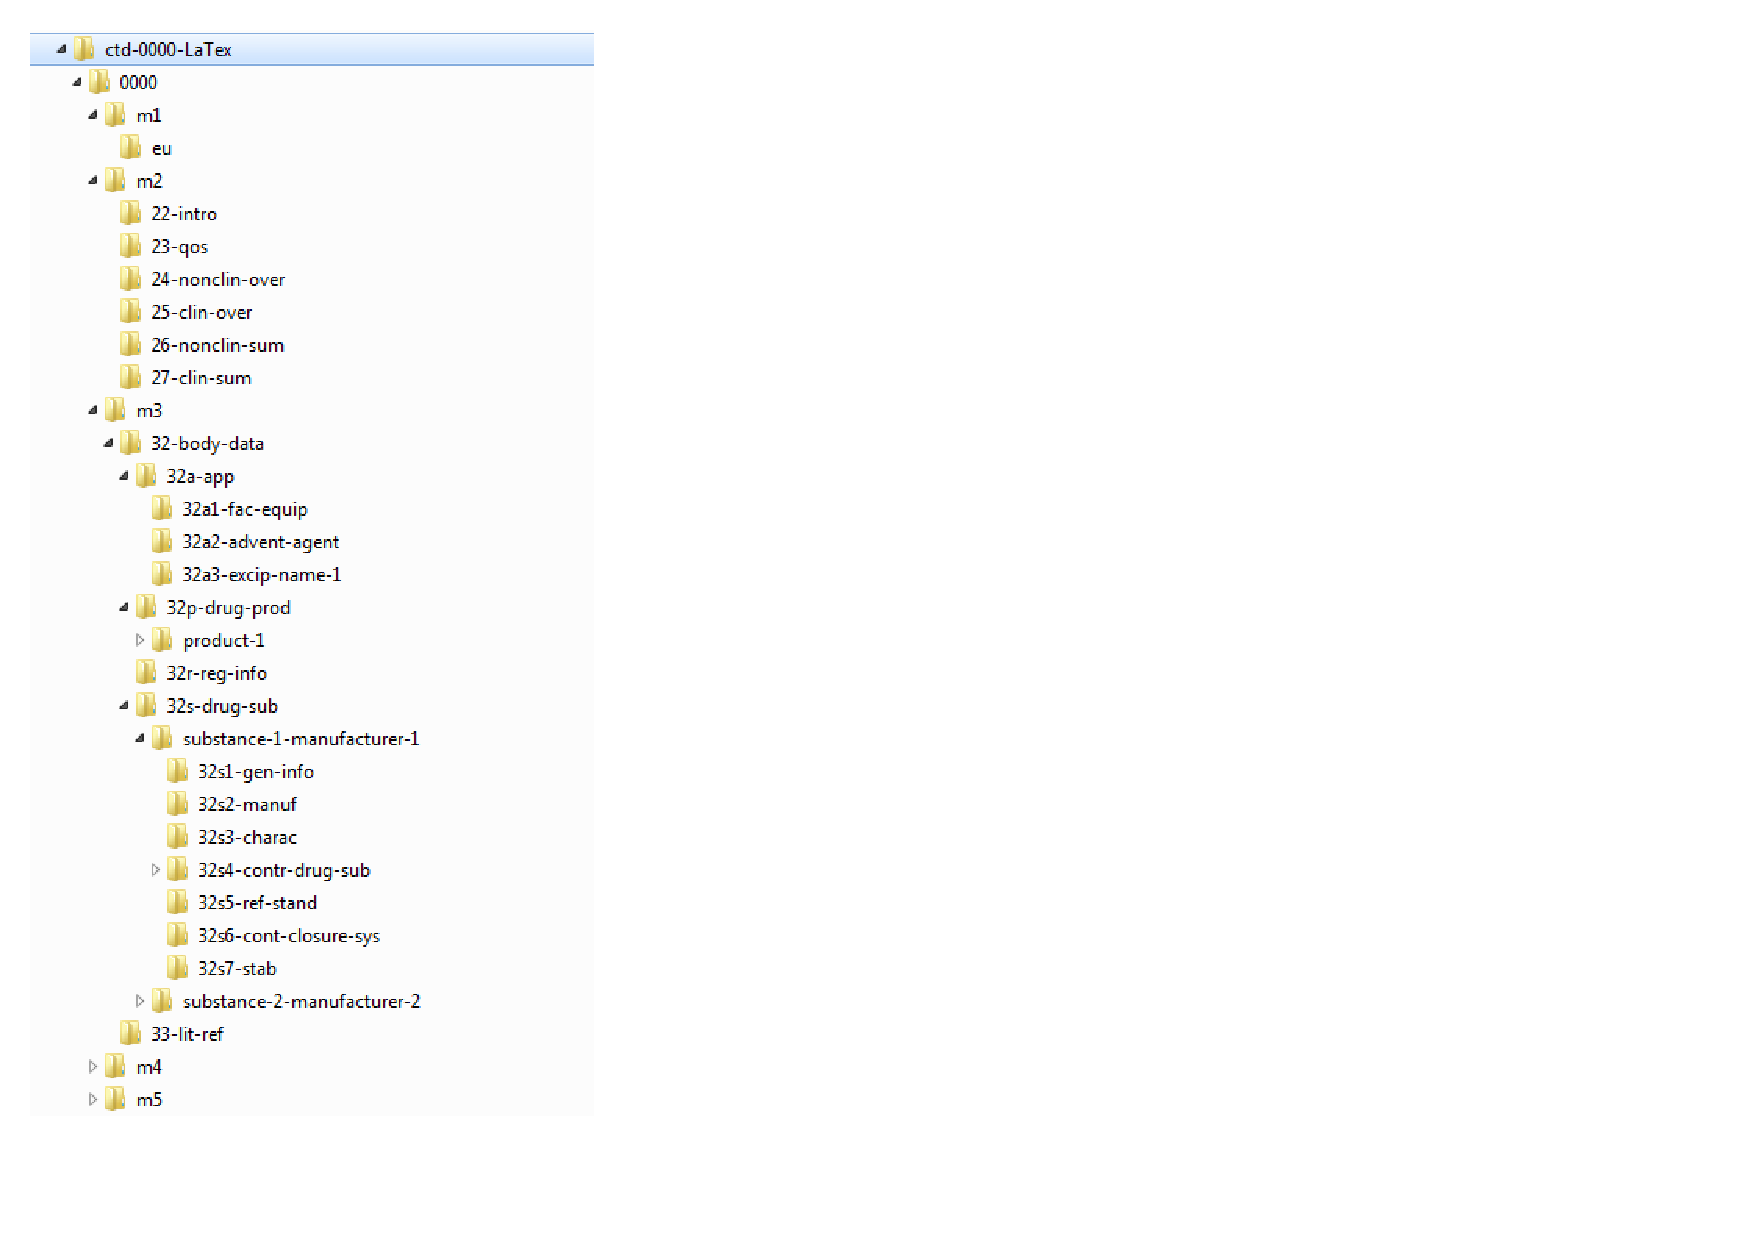
\includegraphics[width=1.5\linewidth]{LatexCTD}
\caption{Organizing of \LaTeX{} Files in an eCTD File and Folder Structure}
\label{fig:eCTDstructure}
\end{figure}

\todo{an BJ: Subfolder mit CTD Example-Datei erzeugen und als screenshot-Figure einbinden}

\section{Extra Packages which are recommended, but which are not included into \PharmRep}
\subsection{Structural Formula of Chemicals with Package \pkg{chemfig}}
To draw molecules and reaction schemes different packages can be used, \eg with package \pkg{chemfig}
something like that:
\bigskip

\chemfig{ * 6((-HO)-=-(-(<[::60]OH)-[::-60]-[::-60,,,2]
HN-[::+60]CH_3)=-(-HO)=)}

\bigskip

\subsection{Graphs and Plots with Package \pkg{TikZ}}
One of the most powerful packages to create graphs and plots is \pkg{TikZ} which can be used for nearly every 
kind of graphical representation, \eg flowcharts, mathematical graphs, 3D visualization, etc. See 
\url{http://www.texample.net/tikz/examples/} for a gallery of examples.
\begin{figure}[hbpt]
\begin{tikzpicture}[%
>=stealth,%
iron/.style={shade, ball color=red},%
electron/.style={shade, ball color=black},%
oxygen/.style={shade, ball color=blue},%
droplet/.style={ball color=blue!20, opacity=0.4},%
]%
% Draw the iron atoms%
\foreach \x in {1,1.5,2,2.5,3,3.5,4,4.5,5,8}%
\draw [iron] (\x,1,-0.5) circle (0.25cm);%
\foreach \x in {1.25,1.75,2.25,2.75,3.25,3.75,4.25,4.75,5.25,5.75,6.25,6.75,7.25,7.75}%
\draw [iron] (\x,0.55,-0.5) circle (0.25cm);%
% Draw the iron electrons; this isn't totally realistic for illustrating Fe+3 ions%
\foreach \x in {1.25,1.75,2.25,2.75}%
\draw [electron] (\x,1.25,-0.5) circle (0.1cm);%
\foreach \x in {1,1.5,2,2.5,3,3.5,4,4.5,5,5.5,6,6.5,7,7.5,8}%
\draw [electron] (\x,0.75,-0.5) circle (0.1cm);%
% Draw the O2 molecules%
\draw [oxygen] (1.5,1.8,-0.5) circle (0.15cm);%
\draw [oxygen] (1.6,2.0,-0.5) circle (0.15cm);%
\draw [oxygen] (1.8,1.6,-0.5) circle (0.15cm);%
\draw [oxygen] (2.05,1.6,-0.5) circle (0.15cm);%
% Draw the arrows showing the electrons going to the O2 molecules%
\draw (3.45,1.35) -- (3.75,2.25) [->,thick];%
\draw (3.95,1.35) -- (3.95,2.25) [->,thick];%
\draw (4.45,1.35) -- (4.35,1.85) [->,thick];%
\draw (4.95,1.35) -- (4.5,1.85) [->,thick];%
% Draw O-2 ions with (-) labels%
\shadedraw [oxygen] (3.75,2.4,-0.5) circle (0.15cm) node [above=3pt,right=2pt] {\small{2-}};%
\shadedraw [oxygen] (4.15,2.0,-0.5) circle (0.15cm) node [above=3pt,right=2pt] {\small{2-}};%
% Draw the dissolved Fe+3 ions and O-2 ions%
\shadedraw [iron] (6.25,2.5,-0.5) circle (0.25cm) node [above=3pt,right=4pt] {\small{3+}};%
\shadedraw [iron] (6.85,2.0,-0.5) circle (0.25cm) node [above=3pt,right=4pt] {\small{3+}};%
\shadedraw [oxygen] (6.95,1.5,-0.5) circle (0.15cm) node [above=3pt,right=2pt] {\small{2-}};%
\shadedraw [oxygen] (6.15,2.0,-0.5) circle (0.15cm) node [above=3pt,right=2pt] {\small{2-}};%
\shadedraw [oxygen] (7.05,2.5,-0.5) circle (0.15cm) node [above=3pt,right=2pt] {\small{2-}};%
% Draw the time arrows%
\draw (2.2,2.5) -- (3.35,2.5) [->,very thick];%
\draw (4.8,2.5) -- (6.15,2.5) [->,very thick];%
% Draw the water droplet%
\begin{scope}%
\clip (1,1) rectangle (8.5,5);%
\draw[droplet] (4.5,1,-0.5) circle (3.5cm);%
\end{scope}%
\end{tikzpicture}
\caption[TikZ example graph rusting iron]{TikZ example graph rusting iron,
\url{http://www.texample.net/tikz/examples/rusting-iron/}}
\end{figure}

\printnoidxglossary[title={List of Abbreviations}]\label{glossari}

\newpage

\appendix
\section{Short List of Common Commands}

Table generated by Excel2LaTeX from sheet `Tabelle1'

{\small
\todo{'Appendix Nummerierung 'A'/ A.1. etc. und in ToC übernehmen}
\begin{tabularx}{\linewidth}{lX}
\textbf{Command} & \textbf{Result}\\
\cs{section\marg{title}} & starts a new section \\
\cs{subsection\marg{title}} & starts a new subsection \\
\cs{subsubsection\marg{title}} & starts a new subsubsection \\
\cs{paragraph\marg{title}} & starts a new paragraph \\
\cs{label\marg{key}} & defines label (must be unique throughout document)\\
\cs{ref\marg{key}} & references label \\
\cs{autoref\marg{key}} & references label and type of reference \\
\cs{pageref\marg{key}} & references pagenumber of label \\
\cs{autopageref\marg{key}} & references pagenumber of label and type of reference \\
\cs{textbf\marg{text}} & bold text \\
\cs{textit\marg{text}} & italic text \\
\cs{small\marg{text}} & small text \\
\cs{footnotesize\marg{text}} & footnotesize text \\
\cs{\%} & percent (\%) \\
\cs{\&} & ampersand (\&) \\
\cs{url\marg{URL}} & url \\
\cs{href\marg{URL}\marg{text}} & text instead of url \\
\cs{landscape} & page orientation landscape \\
\cs{portrait} & page orientation portrait \\
\cs{captionof\{table\}\marg{title}} & caption of table \\
\cs{captionof\{figure\}\marg{title}} & caption of figure \\
\cs{begin\{tabular\}} & simple table \\
\cs{begin\{tabularx\}} & table with automatic width and optional pagebreaks \\
\cs{begin\{figure\}} & figure environment (floating) \\
\cs{includegraphics\marg{filename}} & include `figure' (format png, jpg or pdf) \\
\cs{begin\{itemize\}} & bullet point list \\
\cs{begin\{enumerate\}} & numbered list \\
\cs{item} text & item in list \\
\cs{begin\{description\}} & description list \\
\cs{item[label]} text & item with label (description list only) \\
\cs{input\marg{filename.tex}} & copy-paste contents of tex-file \\
\cs{todo\marg{text}} & comment or todo \\
\cs{cite\marg{bibkey}} & citation of source stored with `bibkey' (in `filename'.bib) \\
\cs{newglossaryentry\marg{glskey}\marg{...}\marg{...}} & define new glossary entry (at the beginning of the \TeX{} file) \\
\cs{gls\marg{glskey}} & use abbreviation stored with `glskey' \\
\end{tabularx}}
\end{document}
%</manual>
%<*manualbib>
@ELECTRONIC{Q1E,
    author = {{International Conference on Harmonization}},
    shorthand = {{International Conference on Harmonization (2004)}},
    month = {6},
    year = {2004},
    title = {Guidance for Industry: Q1E Evaluation of Stability Data.},
    url = 
    {http://www.fda.gov/downloads/Drugs/GuidanceComplianceRegulatoryInformation/Guidances/UCM073380.pdf},
    urldate = {2014-06-28},
    owner = {Barbara Bredner},
    timestamp = {2014.07.10}
}

@BOOK{Berndt2008,
    title={LaTeX. Eine typographische Einf{\"u}hrung.},
    shorthand = {Berndt (2008)},
    author={Tobias Berndt},
    publisher={Addison Wesley},
    year={2008},
    isbn={9783827326591},
    owner={Barbara Bredner},
    timestamp={2014.07.11},
}

@BOOK{Krishnamoorthy,
    title = {Statistical Tolerance Regions: Theory, Applications, and Computation},
    shorthand = {Krishnamoorthy (2009)},
    publisher = {Wiley},
    year = {2009},
    author = {Kalimuthu Krishnamoorthy and Thomas Mathew},
    isbn = {9780470380260},
    owner = {Barbara Bredner},
    timestamp = {2014.05.13},
    totalpages = {461}
}

@BOOK{MontgomeryQC2012,
    title = {Introduction to Statistical Quality Control},
    publisher = {Wiley},
    year = {2012},
    author = {Douglas C. Montgomery},
    edition = {7},
    isbn = {9781118146811},
    owner = {Barbara Bredner},
    timestamp = {2013.06.14},
    totalpages = {768}
}

@ELECTRONIC{EBE,
    author = {{European Biopharmaceutical Enterprises}},
    month = {03},
    year = {2013},
    title = {Considerations in Setting Specifications},
    organization = {{European Biopharmaceutical Enterprises} (EBE)},
    address = {Leopold Plaza Building, Rue du Tr{\^o}ne 108, BE-1050 Brussels},
    url = {http://www.ebe-biopharma.eu/documents/47/25/Considerations-in-Setting-Specifications},
    urldate = {2014-07-11},
    owner = {Barbara Bredner},
    pages = {1-26},
    timestamp = {2014.05.13}
}
%</manualbib>
%<*template>
%% !TeX TXS-program:bibliography = txs:///biber
%%
%% Files required for compilation:
%% literatur.bib
%% TestFlowChart.pdf
%%
%% Compilation in TeXStudio including bibliography and other lists:
%% Press keys in the following order:
%% F6 (compile document)
%% F11/F8 (compile bibliography)
%% If remove one % from the first line biber will be used automatically.
%% F6 (merge document and bibliography as well as other lists)
%%
%%---------------------------------------------

\documentclass{pharmrep}

%%% Load your own LaTeX packages (if really necessary)
\usepackage{blindtext}

%%% Declaration of user and file information
\Applicant{Testpharma Inc.}
\DrugProduct{Test Drug 500mg Tablets}
\PharmRepTitle{3.2.S.x.y Quality Documentation -- Example with usual Layout-Settings}
\eCTDno{eCTD Sequence Number 0001} 
\BibFileName{literatur.bib} % Name of the bibliography file with extension .bib, e.g. 
% biblio.bib


%%% define entries for glossary:
\newglossaryentry{gls:ICH}{name={ICH},description={International Conference on Harmonisation of 
Technical Requirements for Registration of Pharmaceuticals for Human Use}}

\begin{document}
%%%%%%%%%%%%%%%%%
% Start of Text %
%%%%%%%%%%%%%%%%%

\section{First section}
Put your text here


\printnoidxglossary[title={List of Abbreviations}]% not printed until at least 1 abbreviation is used in text
\printbibliography% not printed until at least 1 citation is used in text
\end{document}
%</template>
%\fi